\documentclass[a4paper, oneside, openany,12pt]{article}

% Margini
\usepackage[top=3.1cm, bottom=3.1cm, left=2.2cm, right=2.2cm]{geometry}
\usepackage[utf8]{inputenc}
\usepackage{hyperref}

\usepackage{lastpage}
\usepackage{fancyhdr}
\fancyhf{}
\pagestyle{fancy}
\lhead{Capacity Plan}
\rhead{}
\rfoot{Pagina \thepage{} di \pageref{LastPage}}


\usepackage{graphicx} 		% per immagini
\usepackage{caption}        %numerazione figure e loro descrizione testuale
\usepackage{subcaption}  %sottofigure numerabili
\usepackage{color}
\usepackage[table,xcdraw]{xcolor}
\usepackage{listings}

% Comandi C, L e R per tabelle
\usepackage{array}
\newcolumntype{L}[1]{>{\raggedright\let\newline\\\arraybackslash\hspace{0pt}}m{#1}}
\newcolumntype{C}[1]{>{\centering\let\newline\\\arraybackslash\hspace{0pt}}m{#1}}
\newcolumntype{R}[1]{>{\raggedleft\let\newline\\\arraybackslash\hspace{0pt}}m{#1}}
% Aumenta spaziatura tra righe
\renewcommand\arraystretch{1.5}

% Ref al nome della sezione
\usepackage{nameref}


\title{\textbf{Capacity Plan}}
\author{Lisa Parma}

\begin{document}
	
\begin{titlepage}
	\begin{center}
	
		\textbf{Università degli Studi di Padova \\ Corso di laurea in Informatica \\ Anno 2018-19 \\}
		\textbf{Progetto del corso Amministrazione di Sistema}
		\vspace{1cm}
		\begin{center}
			\begin{figure}[h!]
				\centering
				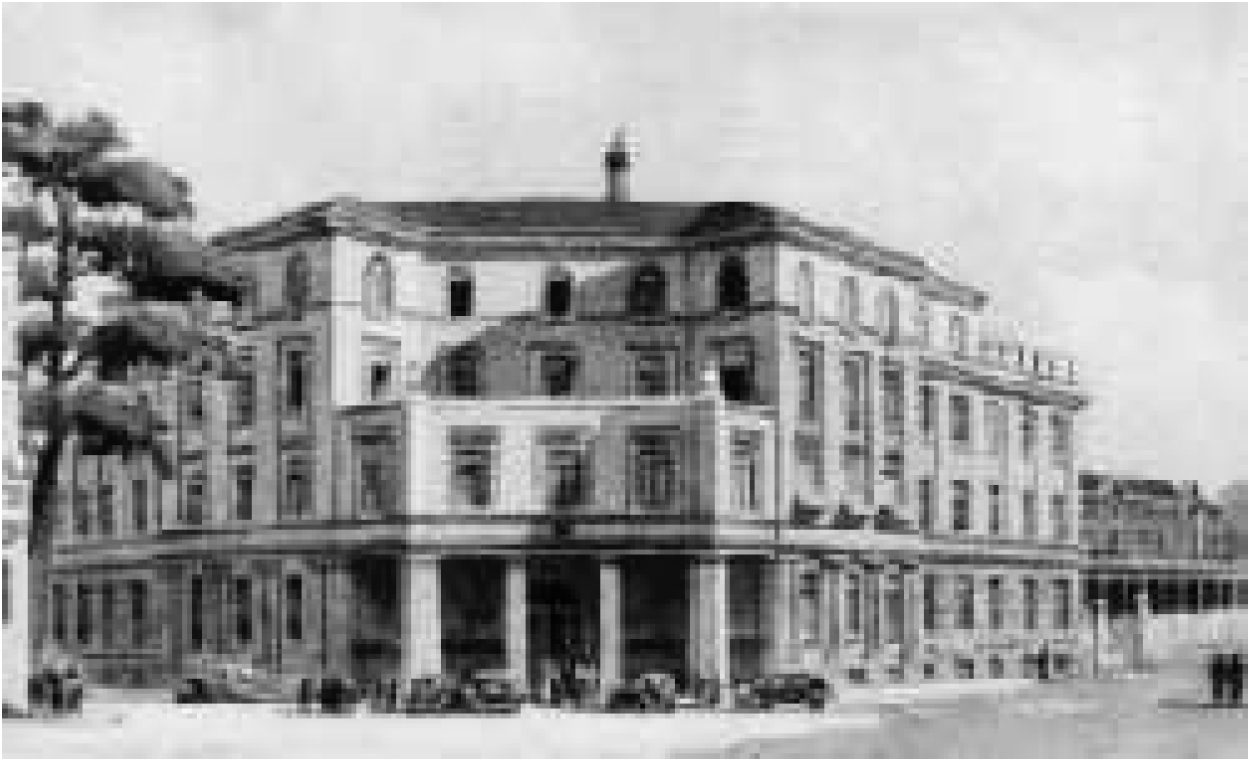
\includegraphics[width=0.5\linewidth]{./img/logo.jpg}
			\end{figure}
			\begin{Huge}
				\textbf{Capacity Plan} \\
			\end{Huge}
			\begin{Large}
				\textbf{Azienda Ospedaliera} \\
				\textbf{Istituto Ortopedico Gaetano Pini} \\
			\end{Large}
		
	\end{center}
	\end{center}
\end{titlepage}

\tableofcontents
\phantomsection
\pdfbookmark{\listtablename}{lot}
\listoftables
% SEZIONI DEL DOCUMENTO
% qui vanno presentate in ordine di apparizione le sezioni che compongono il documento
\newpage
	\newpage

\section{Introduzione}
	Con il presente documento si vuole fornire una stima delle risorse IT necessarie per supportare le funzionalità e i requisiti di prestazione delle varie applicazioni utilizzate e servizi forniti dall'istituto  Ospedaliero Gaetano Pini.\\
	Il piano di capacità tiene conto dei servizi e delle tecnologie utilizzate ad oggi e delle previsioni della domanda dell'istituto, stimando costi per il raggiungimento degli obbiettivi concordati in termini di livello di servizio.
	Le stime effettuate sono frutto dell'osservazione dell'attuale sistema.
	
	\subsection{Struttura documento}
	Il seguente documento è strutturato come segue:
	\begin{itemize}
		\item La sezione 2, Scenario aziendale, elenca la struttura ad oggi dei servizi e delle infrastrutture tecnologiche utilizzate, ne descrive il campo applicativo, l'utilizzo e la criticità.
		\item La sezione 3, Analisi di capacità, analizza le informazioni della precedente sezione e i piani di crescita in modo da poter determinare i requisiti di capacità, considerando scalabilità, velocità, disponibilità e sicurezza.
		\item 
		\item
	\end{itemize}
	
	\subsection{Assunzioni}
	Le assunzioni effettuate 
	\newpage

\section{Scenario aziendale}
	\textcolor{red}{In questo paragrafo verrà descritta l'attuale situazione dell'organizzazione di servizio e della disponibilità di sistemi  }
	\subsection{Sistemi applicativi esistenti}
	La seguente tabella descrive i servizi applicativi centralizzati tutt’ora utilizzati per far fronte alle attività dell’istituto. \\
	Ogni riga della tabella contiene un applicativo e per ogni uno viene specificato:
	\begin{itemize}
		\item criticità, indicata con un numero che va da 1 a 5 e definita dall'istituto,;
		\item numero di utenti totali che utilizzano quel determinato applicativo;
		\item numero di utenti che utilizzano quell'applicativo in contemporanea;
		\item servizio per il quale quell'applicativo viene utilizato;
		\item criticità del servizio indicata con un numero che va da 1 a 5.
	\end{itemize}
	\begin{table}[h]
		\begin{tabular}{|c|C{3cm}| C{2cm} |C{1.5cm} |C{2cm} | C{3cm} | C{2cm}|}
			\hline
			\rowcolor[HTML]{EFEFEF} 
			\textbf{N} & \textbf{Sistema applicativo}  & \textbf{Criticità (1-5)} & \textbf{N. utenti} & \textbf{N. utenti attivi}  & \textbf{Servizio} & \textbf{Criticità servizio (1-5)}\\ \hline
			1  & Archivio Clinico		& 4		& 15	& 10 		& Gestione archivio clinico & 4		\\ \hline
			2  & Argos						& 4		& 5	 		& 2 		& Valorizzazione dei DRG & 3		\\ \hline
			3  & Armonia					& 4		& 6		& 3 		& Gestione anatomia patologica & 4		\\ \hline
			4  & Emonet						& 4		& 10	& 2 		& Gestione produzione emoderivanti & 5		\\ \hline
			5  & Aurora Web				& 2		& 650	& 100 		& Gestione pazienti  & 5		\\ \hline
			6  & Gst\_est					& 2		& 650	& 20 		&  & 		\\ \hline
			7  & Gst\_fat					& 2		& 6			& 4 		& Gestione fatturazione & 4		\\ \hline
			8  & Pacs						& 2		& 49		& 20 		& Gestione diagnostica per immagini & 5	\\ \hline
					9  & Elefante					& 2		& 49		& 20 		&  & 		\\ \hline
		\end{tabular}
	\end{table}

	\begin{table}[h]
	\begin{tabular}{|c|C{3cm}| C{2cm} |C{1.5cm} |C{2cm} | C{3cm} | C{2cm}|}
		\hline
		\rowcolor[HTML]{EFEFEF} 
\textbf{N} & \textbf{Sistema applicativo}  & \textbf{Criticità (1-5)} & \textbf{N. utenti} & \textbf{N. utenti attivi}  & \textbf{Servizio} & \textbf{Criticità servizio (1-5)}\\ \hline
		10  & Ormawin2000		& 4		& 6			& 3 		& Gestione sale operatorie / materiale protesico & 3		\\ \hline
		11  & PowerLab				& 2		& 10		& 5 		& Gestione laboratorio analisi & 5		\\ \hline
		12  & Rap						& 3		& 6			& 4 		& Gestione fatturazione & 4		\\ \hline
		13  & Ican						& 2		& 350 		& 100 		& Piattaforma SISS & 4		\\ \hline
		14  & Aliseo					& 4		& 20 		& 5 		& Gestione delle risorse umane & 4	\\ \hline
		15  & Enco						& 4		& 43 		& 20 		& Gestione amministrazione e magazzini & 4	\\ \hline
		16  & Teseo						& 2		& 10 		& 2 		&  & 	\\ \hline
		17  & Protocollo			& 3		& 15 		& 5 		& Gestione protocollo & 3	\\ \hline
	\end{tabular}
\end{table}

	\subsection{Infrastrutture tecnologiche esistenti}


	\begin{table}[h]
	\begin{tabular}{|l|l|l|l|l|}
		\hline
		\rowcolor[HTML]{EFEFEF} 
		\textbf{N} & \textbf{Sistema applicativo}  & \textbf{Criticità} & \textbf{Numero utenti} \\ \hline
		1  & Router internet	& 4		& 15		\\ \hline
		2  & Argos		& 4		& 5		\\ \hline
		3  & Armonia		& 4		& 6		\\ \hline
		4  & Emonet				& 4		& 10		\\ \hline
		5  & Aurora Web		& 2		& 650		\\ \hline
		6  & Gest\_est			& 2		& 650		\\ \hline
		7  & GES\_fat			& 2		& 6		\\ \hline
		8  & Pacs		& 2		& 49		\\ \hline
		9  & Elefante		& 2		& 49		\\ \hline
		10  & Oemawin200		& 4		& 6		\\ \hline
		11  & PowerLab						& 2		& 10		\\ \hline
		12  & Rap				& 3		& 6		\\ \hline
		13  & Ican		& 2		& 350 	\\ \hline
		14  & Aliseo			& 2		& 350 	\\ \hline
		15  & Enco		& 2		& 350 	\\ \hline
		16  & Teseo			& 2		& 350 	\\ \hline
		17  & Protocollo			& 2		& 350 	\\ \hline
	\end{tabular}
\end{table}

	
	\newpage
\section{Analisi di capacità}
Questa sezione descrive gli scenari analizzati in termini di impatto sui processi aziendali in modo da poter determinare con precisione i requisiti di capacità. Considerare la scalabilità, la velocità effettiva, i requisiti di disponibilità, l'archiviazione, l'utilizzo delle risorse, la sicurezza, i backup, ecc. E, se del caso, delineare la strategia per lo sviluppo di questi scenari.
Descrivere i piani di crescita e come verranno affrontati e gestiti. Considerare non solo i requisiti per hardware, software, materiali da costruzione e spazio aggiuntivi, ma anche da dove provengono finanziamenti finanziari per queste cose; requisiti aggiuntivi di allocazione delle risorse; personale, formazione, altre spese, ecc. Espandere su questa sezione aggiungendo / rimuovendo scenari aggiuntivi, se necessario.

\subsection{Previsione dell'utilizzo e delle prestazioni del servizio}
	Tutti i dettagli su tutti i livello di servizio monitorati.
	
	\subsubsection{Presupposti}
	Ipotesi su cui si basa la previsione 
	\subsubsection{Previsioni}
	\subsubsection{Misure per far fronte alla domanda aggiuntiva}
	
	
\subsection{Previsione dell'utilizzo e delle prestazioni delle risorse}



\newpage
\section{Analisi di impatto}


\newpage
\section{Analisi del rischio}

\newpage
\section{Costi}

\end{document}